\section{Разработка системы распределенных вычислений}

В данном разделе рассматривается практическая реализация
разработанной системы распределённых вычислений. Описываются
реализация Raft-узла как центрального элемента кластера, устройство
серверного модуля и менеджера заданий, а также конфигурация узлов и
клиентского приложения. Далее приводится описание реализации
вычислительного узла и рассматриваются результаты тестирования
системы, включая проверку отказоустойчивости, корректности
выполнения задач, поведения при конкурентной нагрузке и обработке
задач большого объёма.

Полный исходный код можно найти в \cite{abeille}.

\subsection{Реализация Raft-узла}

Raft-узел является центральным элементом системы: он реализует алгоритм
консенсуса, поддерживает реплицированную машину состояний и предоставляет
интерфейсы для взаимодействия с пользователями и вычислительными узлами.
Реализация узла включает несколько взаимосвязанных компонентов: Raft-лог,
машину состояний с поддержкой снимков данных, серверный модуль, менеджер
заданий и подсистему конфигурации.

\subsubsection{Raft-лог}

Лог Raft представляет собой основной журнал команд, которые подлежат
репликации между всеми узлами кластера. После достижения кворума
запись из лога коммитится и применяется к машине состояний.
В данной реализации поддерживаются две команды:

\begin{itemize}
    \item \texttt{RAFT\_COMMAND\_ADD} — добавление новой задачи в очередь назначенных;
    \item \texttt{RAFT\_COMMAND\_MOVE} — перевод задачи в состояние завершённых.
\end{itemize}

Структура записи лога описана с использованием Protocol Buffers
(см. рис.~\ref{fig:raftlog}). Каждая запись включает тип команды,
номер терма, полезную нагрузку (упакованную в \texttt{TaskWrapper}),
а также дополнительные поля, зависящие от команды
(\texttt{AddRequest} или \texttt{MoveRequest}).
Использование Proto-схемы обеспечивает строгую типизацию,
возможность обратной совместимости при изменении формата и
автоматическую генерацию сериализаторов/десериализаторов.

\begin{figure}[h!]
    \centering
    \includegraphics[width=0.6\linewidth]{inc/raft_log_entry.png}
    \caption{Структура записи Raft-лога, определённая в формате Protocol Buffers.}
    \label{fig:raftlog}
\end{figure}

С точки зрения реализации лог представляет собой потокобезопасную обёртку над
\texttt{std::deque}. Такой выбор объясняется необходимостью обеспечения:

\begin{itemize}
    \item Быстрого случайного доступа по индексу (для алгоритма согласования);
    \item Эффективного удаления элементов как из начала
    (очистка закоммиченных записей после создания снимка данных),
    так и из конца (откат неконсистентных записей при пересинхронизации).
\end{itemize}

Индексация в логе начинается с $1$; нулевой индекс считается невалидным и
используется для упрощения проверок корректности ссылок на записи.

\subsubsection{Машина состояний и механизм снимка данных}

Машина состояний реализует детерминированный автомат, который постепенно
применяет закоммиченные записи лога и формирует текущее состояние кластера. Она
хранит:

\begin{itemize}
    \item список назначенных задач;
    \item список завершённых задач;
    \item текущий номер терма и индекс последней применённой команды.
\end{itemize}

Для предотвращения бесконтрольного роста размера лога реализован механизм
снимков данных (snapshotting). При достижении порога, заданного
пользователем в конфигурационном файле, машина состояний инициирует создание
снимка данных: сериализует своё текущее состояние и сохраняет его на диск. Данный
процесс выполняется асинхронно, что позволяет продолжать применение новых
команд без блокировки. После успешной записи снимка данных лог очищается от записей,
которые были зафиксированы в сохранённом состоянии, что ограничивает его размер
сверху.

В случае, если лидер не находит в своём логе необходимой записи для
синхронизации с отстающим узлом, он инициирует передачу ему актуального
снимка данных, после чего узел может восстановить своё состояние и продолжить
репликацию с последнего зафиксированного индекса.

\subsection{Серверный модуль}

Серверный модуль представляет собой важный компонент всей системы,
отвечающий за приём, маршрутизацию и первичную обработку входящих сетевых
запросов. Его основная задача — служить универсальной точкой входа для
различных внешних и внутренних участников распределённой системы.

Функционально сервер инкапсулирует gRPC-сервер — высокопроизводительный и
расширяемый сетевой стек, построенный на современных RPC-технологиях. Это
позволяет обеспечить устойчивую и быструю обработку запросов с минимальной
задержкой, а также обеспечивает возможность масштабирования на кластеры узлов.

Сервер принимает запросы от трёх ключевых источников:
\begin{itemize}
    \item других узлов (сервис \texttt{RaftService}: \texttt{RequestVote()},
    \texttt{AppendEntries()}, \texttt{InstallSnapshot()});
    \item клиентов (сервис \texttt{UserService});
    \item вычислительных узлов (сервис \texttt{WorkerService}).
\end{itemize}

\begin{itemize}
    \item \texttt{Сервис RaftService} — используется для взаимодействия между
        различными узлами кластера. Через него проходят критически важные
        RPC-вызовы, обеспечивающие функционирование алгоритма консенсуса Raft,
        такие как:
    \begin{itemize}
        \item \texttt{RequestVote()} — инициирует процедуру голосования при
            выборах лидера;
        \item \texttt{AppendEntries()} — используется лидером для
            распространения изменений в журнале (log replication);
        \item \texttt{InstallSnapshot()} — применяется для инициации снимка данных.
    \end{itemize}

    \item \texttt{Сервис UserService} — предназначен для взаимодействия с
        пользовательскими интерфейсами. Запросы, поступающие от клиентов,
        обрабатываются в рамках общего бизнес-процесса и могут содержать как
        команды на изменение состояния, так и запросы на получение данных.

    \item \texttt{Сервис WorkerService} — обеспечивает коммуникацию с
        вычислительными узлами, выполняющими задачи в рамках более широкой
        архитектуры.
\end{itemize}

Сервер маршрутизирует запросы: приём запросов на запись выполняется любым
узлом, но при отсутствии лидерства происходит перенаправление клиента на лидера
путем посылки ему ответа \texttt{REDIRECT}.

\subsection{Менеджер заданий}

Task Manager отвечает за подготовку записей для лога Raft при добавлении и
завершении задач, а также за передачу результата пользователю. В реализации
предусмотрены три основных метода:

\begin{itemize}
    \item \texttt{UploadTaskData} — получает данные задачи, выбирает
    идентификатор рабочего узла через \texttt{WorkerServiceImpl::AssignTask()}
    и формирует запись с командой \texttt{RAFT\_COMMAND\_ADD}.
    После успешного выбора рабочего узла запись добавляется в лог Raft
    для репликации и последующего применения к машине состояний.
    \item \texttt{ProcessTask} — передаёт задачу на исполнение выбранному рабочему узлу.
    \item \texttt{UploadTaskResult} — формирует команду
    \texttt{RAFT\_COMMAND\_MOVE}, переводящую задачу из статуса
    \emph{assigned} в \emph{completed}, и добавляет её в лог для
    репликации и коммита.
    \item \texttt{SendTaskResult} — отправляет готовый результат
    обратно в \texttt{UserServiceImpl} для передачи клиенту.
\end{itemize}

Следует отметить, что назначение задачи на рабочего узла выполняется ровно один раз в
момент вызова \texttt{UploadTaskData}. В текущей версии реализации не
предусмотрен механизм автоматического перевыбора рабочего узла или повторной выдачи
задачи при сбое, однако согласованность и идемпотентность обеспечиваются за
счёт самого алгоритма Raft: если запись не была закоммичена до отказа лидера,
она не будет применена к машине состояний, и задача может быть отправлена
повторно клиентом.

\subsubsection{Конфигурация и инициализация узла}

Перед запуском узла пользователь должен предоставить
JSON-конфигурацию (см. рис.~\ref{fig:raftconfig}), в которой указываются:
\begin{itemize}
    \item адреса сервисов (пользовательский, рафт-сервис, сервис рабочего);
    \item список адресов всех узлов кластера (включая данный узел);
    \item параметр \texttt{snapshot\_after} — количество коммитов
    до создания нового снимка данных;
    \item путь к файлу, куда будет записываться снимок данных.
\end{itemize}

\begin{figure}[h!]
    \centering
    \includegraphics[width=0.65\linewidth]{inc/raft_config_example.png}
    \caption{Пример конфигурационного файла Raft-узла.}
    \label{fig:raftconfig}
\end{figure}

В коде конфигурация инкапсулирована в синглтон-объект, который доступен всем
компонентам узла, что упрощает инициализацию и исключает дублирование настроек.
Приложение также поддерживает переопределение некоторых параметров через
аргументы командной строки, что полезно для тестирования и развёртывания в
разных окружениях.

\subsubsection{Конфигурация клиента}

Клиентское приложение предоставляет пользователю консольный интерфейс для
постановки задач на выполнение в кластер и получения результатов. Его
функциональность разбита на несколько подсистем: загрузка конфигураций,
подготовка задания, взаимодействие с кластером, ожидание/получение результата и
сохранение артефактов.

Клиентское приложение конфигурируется с помощью трех файлов. Первый из них
содержит перечень известных адресов узлов Raft. Пример привден на
рис~\ref{fig:client_config}.

\begin{figure}
  \centering
  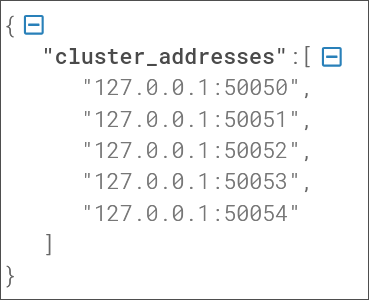
\includegraphics[scale=0.4]{inc/client-config.png}
  \caption{Пример клиентского конфигурационного файла}
  \label{fig:client_config}
\end{figure}

Клиент инициализирует пул соединений к указанным адресам и выбирает рабочую
«точку входа» по порядку (или по доступности). При ошибке соединения
выполняется следующий адрес из списка, что обеспечивает толерантность к отказу
отдельного узла без участия пользователя. Запросы, изменяющие состояние
(постановка задачи), отправляются на любой доступный узел; при необходимости
выполняется прозрачный редирект на лидера.

Второй файл задаёт путь для сохранения результатов и имя динамической
библиотеки задачи (см. рис.~\ref{fig:user_config})

\begin{figure}
  \centering
  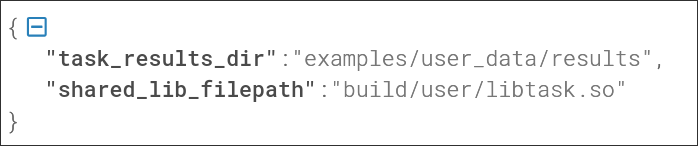
\includegraphics[scale=0.4]{inc/user-config.png}
  \caption{Пример пользовательского конфигурационного файла}
  \label{fig:user_config}
\end{figure}

Третий же файл содержит данные для задания (см. рис.~\ref{fig:user_data}).

\begin{figure}
  \centering
  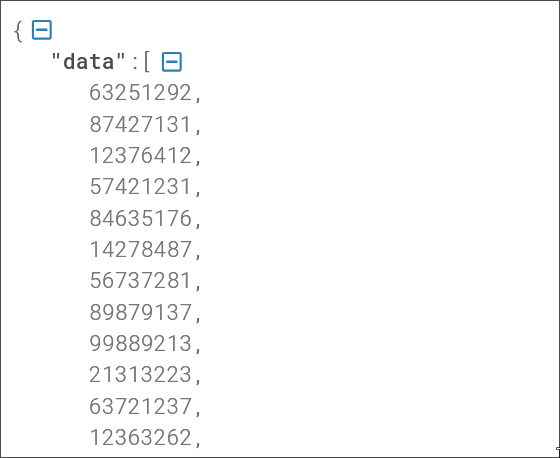
\includegraphics[scale=0.4]{inc/user-data.png}
  \caption{Пример данных для задания}
  \label{fig:user_data}
\end{figure}

\subsubsection{Протокол клиентского приложения}

Взаимодействие клиента с кластером реализовано поверх двунаправленного
потокового вызова \texttt{UserService.Connect}, определённого в gRPC (см.
приложение A, \texttt{User service }). Использование потокового RPC позволяет
поддерживать длительное соединение, через которое клиент и сервер обмениваются
сообщениями в обоих направлениях: клиент отправляет последовательность
запросов, а сервер — последовательность ответов, не прерывая сессию. Такой
подход позволяет объединить обнаружение лидера, постановку задачи и получение
результата в единый непрерывный диалог.

Каждое сообщение клиента содержит поле \texttt{status}, отражающее фазу работы.
На этапе инициализации клиент посылает кадр со статусом \texttt{IDLE},
сигнализируя о готовности к работе. Если узел, на который был направлен запрос,
не является лидером кластера, сервер возвращает ответ с командой \texttt{REDIRECT}
и идентификатором актуального лидера. Получив такую команду, клиент закрывает
поток и устанавливает соединение с указанным узлом, гарантируя, что все
последующие запросы пойдут через единственный согласованный канал.

После установления соединения с лидером клиент переходит к передаче данных
задачи. Для этого используется статус \texttt{UPLOAD\_DATA}, а в сообщении
указываются полезная нагрузка (например, содержимое входного файла),
логическое имя этой нагрузки и идентификатор динамической библиотеки, которая
будет использована при выполнении задачи. Следует подчеркнуть, что по сети
передаётся только имя библиотеки, а не её бинарный образ, поскольку сами
модули заранее развёрнуты на вычислительных узлах. Сервер принимает эти данные,
реплицирует соответствующую команду в Raft-лог, а после достижения кворума
отправляет клиенту ответ с командой \texttt{ASSIGN}, в котором содержится
сгенерированный идентификатор задачи и подтверждение того, что она принята
кластером.

Соединение не разрывается после постановки задачи, а остаётся открытым до
получения финального результата. Когда задача завершается на рабочем узле, её
результат реплицируется через Raft и фиксируется в машине состояний. Лишь
после этого сервер отправляет клиенту команду \texttt{RESULT}, содержащую
окончательный статус выполнения и, при необходимости, сериализованный результат.
Таким образом, клиент всегда получает согласованное состояние, подтверждённое
кворумом узлов.

В совокупности такой протокол обеспечивает упорядоченный и надёжный обмен:
постановка задачи и выдача результата проходят через единую двунаправленную
сессию, которая переносит всю сложность работы с распределённым кластером на
серверную сторону. Клиенту не требуется отслеживать состояние выборов или
дублировать запросы вручную: редиректы, подтверждения и уведомления о результате
получаются автоматически, что делает взаимодействие простым, но при этом
линейризуемым и устойчивым к сбоям.

\subsection{Реализация вычислительного узла}

Вычислительный узел (worker) предназначен для исполнения задач, поступающих из
кластера, и построен вокруг длительного двунаправленного потокового соединения
\texttt{WorkerService.Connect}. При запуске узел считывает локальную
конфигурацию, в которой указывается каталог для размещения динамических
библиотек (\texttt{libs\_dir}) (пример конфигурации приведен на
рис.~\ref{fig:worker_config}). Этот каталог используется как единое хранилище
исполняемых модулей, на которые ссылаются задания. Клиентская часть передаёт
библиотеку в кластер Raft; после репликации и коммита серверная сторона
распределённой системы доставляет содержимое соответствующего артефакта на
вычислительные узлы, где он сохраняется в \texttt{libs\_dir} и становится
доступным среде исполнения.

\begin{figure}
  \centering
  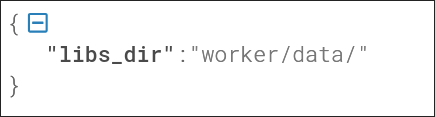
\includegraphics[scale=0.4]{inc/worker-config.png}
  \caption{Пример конфигурационного файла вычислительного узла}
  \label{fig:worker_config}
\end{figure}

Протокол общения вычислительного узла с кластером представлен в приложении А
(см. \texttt{Worker service}). Логика взаимодействия с кластером организована
как непрерывная сессия. Сразу после установления соединения вычислительный узел
отправляет кадр с собственным состоянием \texttt{IDLE}, тем самым сигнализируя
о готовности к приёму работы. Если подключение установлено не с лидером, сервер
немедленно возвращает команду перенаправления с указанием \texttt{leader\_id};
рабочий узел закрывает текущий поток и повторяет подключение к лидеру, после
чего цикл продолжается без участия оператора. В штатном режиме лидирующий
сервер выдаёт команду назначения, в которой указывает идентификатор задачи и,
при необходимости, содержит полезную нагрузку и бинарные данные библиотеки. В
момент получения такого ответа рабочий узел выполняет атомарную подготовку
окружения: проверяет наличие требуемого модуля в \texttt{libs\_dir}, при
отсутствии записывает поступивший образ на диск и синхронно fsync’ит его,
формируя детерминированное имя файла (например, по хешу содержимого или по
имени, пришедшему от сервера), после чего сверяет права доступа и готовность к
загрузке. Этим достигается инвариант, согласно которому перед запуском
пользовательского кода соответствующая библиотека обязательно присутствует
локально и доступна для динамического связывания.

Переход от состояния ожидания к выполнению инициируется командой
\texttt{PROCESS}. Получив её, узел запускает изолированный дочерний процесс
исполняющей среды (в проекте такой процесс может создаваться простым
\texttt{fork()} без сложной контейнеризации), загружает динамическую библиотеку
из \texttt{libs\_dir} и вызывает заранее оговорённый символ интерфейса,
передавая входные данные из \texttt{task\_data}. Основная служба рабочего узла при
этом остаётся в состоянии «занят» и периодически отправляет в поток
\texttt{WorkerConnectRequest} собственный статус и актуальную проекцию
\texttt{TaskState}, обеспечивая наблюдаемость прогресса. В случае штатного
завершения исполняющий процесс формирует результат и отдаёт его основному
процессу узла; далее результат включается в \texttt{TaskState} и возвращается в
кластер тем же потоковым соединением. После этого вычислительный узел переводит
себя в состояние \texttt{COMPLETED}, что служит для серверной стороны сигналом
о готовности зафиксировать завершение в реплицированной машине состояний и
инициировать доставку результата клиенту.

Особое внимание уделено устойчивости к частичным сбоям. Если в ходе выполнения
падает дочерний процесс или попытка динамической загрузки модуля завершается
ошибкой, основная служба не теряет связь с кластером: рабочий узел немедленно
фиксирует ошибочное завершение в \texttt{TaskState} и отправляет его через
активный поток, после чего возвращается в состояние \texttt{IDLE}. Повторы
команд со стороны сервера не приводят к дублированию работы: задача
идентифицируется по \texttt{task\_id}, поэтому рабочий узел либо игнорирует повторные
\texttt{PROCESS} для уже завершённой задачи, либо корректно восстанавливает
исполнение, если сбой произошёл до выдачи финального состояния. Аналогично
сетевые разрывы и смена лидера обрабатываются на транспортном уровне: поток
может быть закрыт с соответствующим статусом gRPC, после чего узел повторяет
подключение с публикацией своего фактического состояния, а серверная сторона,
опираясь на зафиксированные в Raft переходы, восстанавливает согласованную
картину происходящего.

Таким образом, вычислительный узел реализует минимально необходимую
инфраструктуру для безопасного исполнения пользовательского кода: чтение
конфигурации и подготовка каталога библиотек; устойчивое потоковое соединение с
лидером кластера; детерминированная подготовка исполняемого окружения и
загрузка модулей из \texttt{libs\_dir}; изоляция пользовательского исполнения в
отдельном процессе; регулярная публикация статуса и финализация результата
через \texttt{WorkerService.Connect}. Все переходы по состояниям рабочего узла
(\texttt{IDLE} $\rightarrow$ \texttt{BUSY} $\rightarrow$ \texttt{COMPLETED})
отражаются в потоке запросов, а сервер отвечает соответствующими командами
управления и данными (\texttt{ASSIGN}, \texttt{PROCESS}, \texttt{REDIRECT}),
сохраняя линейризуемую семантику наблюдения и единый порядок событий для всех
участников системы.

\subsection{Тестирование системы распределенных вычислений}

\subsubsection{Тестирование отказоустойчивости}

Проверка корректности реализации алгоритма Raft проводилась с использованием
ручных интеграционных испытаний. Для этого на локальной машине было запущено
три экземпляра Raft-узлов, каждый из которых инициализировался собственной
конфигурацией и прослушивал уникальный TCP-порт. На этапе инициализации узлы
формируют сетевые потоки (\texttt{peer threads}), регистрируют gRPC-сервисы и
начинают обмен heartbeat-сообщениями.

В первом эксперименте система демонстрирует штатное избрание лидера:
через заданный таймаут по истечении срока аренды один из узлов инициировал
выборы (лог содержит сообщение \texttt{Starting election in term 1}) и,
получив кворум голосов, объявил себя лидером (\texttt{I'm the leader now}).
В таком состоянии кластер готов принимать клиентские запросы, а
закоммиченные записи будут реплицироваться на оставшиеся узлы. Лог мастера
изображен на рис.~\ref{fig:leader_log}. Лог одной из реплик же представлен
на рис.~\ref{fig:replica_log}.

\begin{figure}
  \centering
  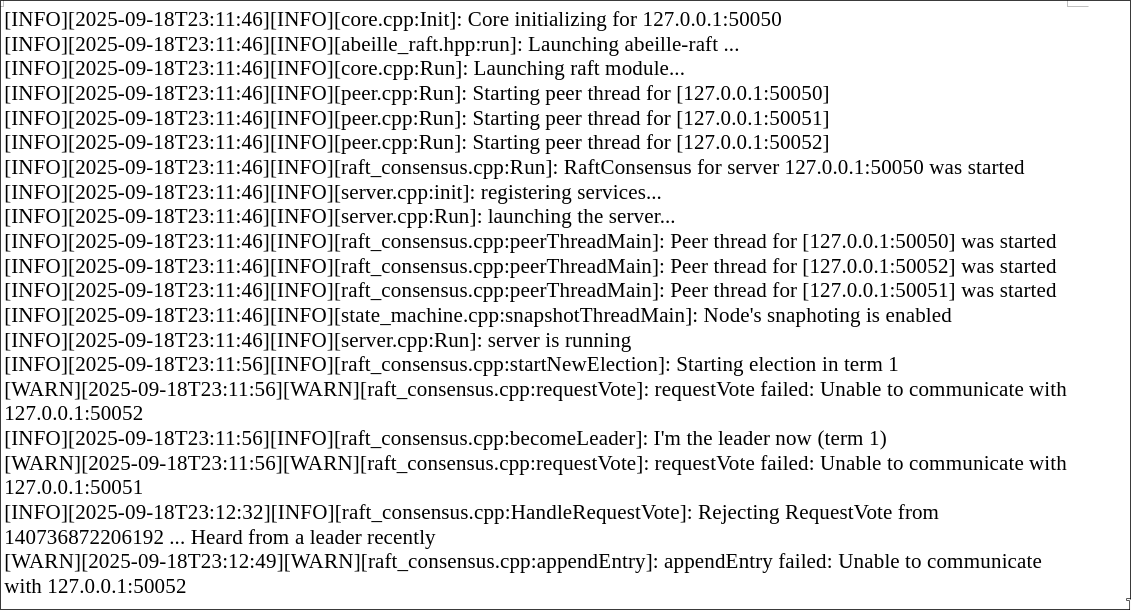
\includegraphics[scale=0.4]{inc/leader-log.png}
  \caption{Лог мастера при первом выборе лидера}
  \label{fig:leader_log}
\end{figure}

\begin{figure}
  \centering
  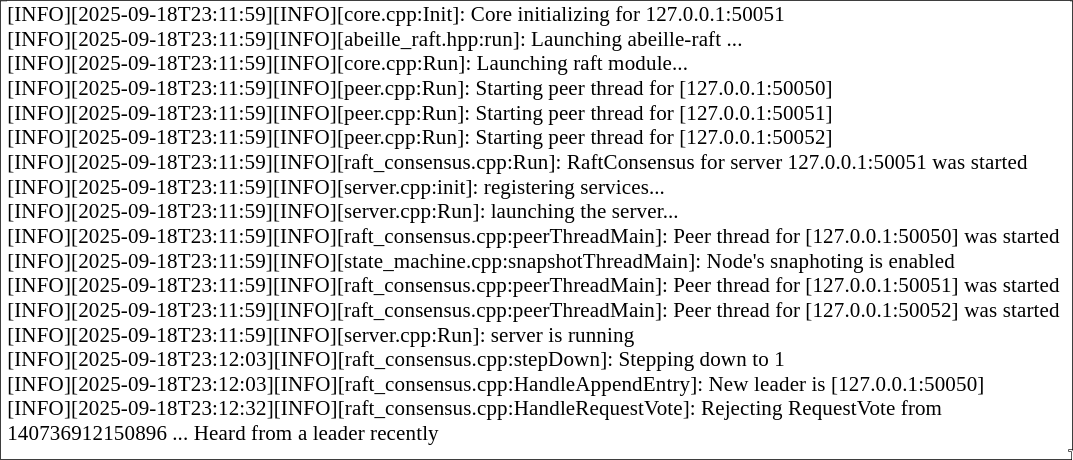
\includegraphics[scale=0.4]{inc/replica-log.png}
  \caption{Лог реплики при первом выборе лидера}
  \label{fig:replica_log}
\end{figure}

Затем моделировался отказ лидера: первый узел был остановлен, что привело к
прекращению рассылки heartbeat-пакетов (см. рис.~\ref{fig:leader-shutdown}).

\begin{figure}
  \centering
  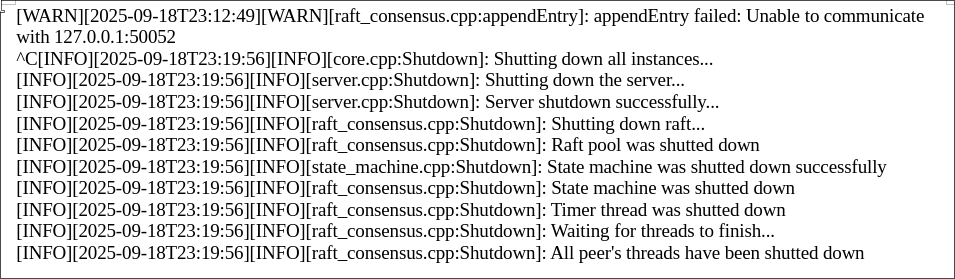
\includegraphics[scale=0.4]{inc/master-after-shutdown.png}
  \caption{Логи при остановке мастера}
  \label{fig:leader-shutdown}
\end{figure}

Спустя период \texttt{election timeout} один из оставшихся узлов инициировал
новый раунд выборов (терм 2), получил поддержку большинства и стал новым
лидером. В логах зафиксировано событие \texttt{becomeLeader} с указанием нового
терма, что подтверждает корректную работу механизма смены лидерства и
сохранение согласованности состояния кластера, это представлено на рис.
~\ref{fig:new-master}.

\begin{figure}
  \centering
  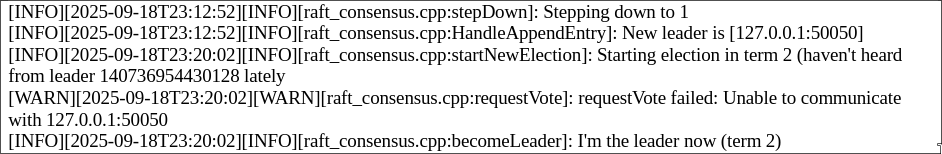
\includegraphics[scale=0.4]{inc/replica-master-after-shutdown.png}
  \caption{Логи нового мастера после остановки старого}
  \label{fig:new-master}
\end{figure}

Процесс голосования реплики за нового лидера представлен на рис.
~\ref{fig:replica-after-new-leader}.

\begin{figure}
  \centering
  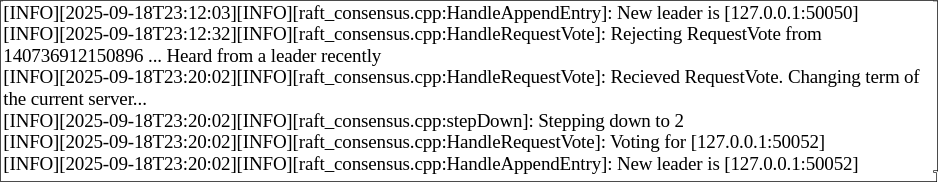
\includegraphics[scale=0.4]{inc/replica-after-shutdown.png}
  \caption{Процесс голосования за нового лидера}
  \label{fig:replica-after-new-leader}
\end{figure}

Такие испытания позволяют убедиться, что система корректно реагирует на сбои:
потеря лидера не приводит к недоступности сервиса, а лишь инициирует повторные
выборы, после которых кластер восстанавливает способность обрабатывать запросы.
В сочетании с механикой репликации и commit-индексов это гарантирует, что все
закоммиченные записи остаются видимыми для клиента даже при перезапуске узлов.

\subsubsection{Инициализация клиентского приложения и подключение к кластеру}

Тестирование вычислительного процесса начинается с запуска консольного клиента
с указанием конфигурационных файлов пользователя и кластера. На
рис.~\ref{fig:client_start} приведён фрагмент журнала запуска клиента. В ходе
подключения клиент последовательно обходит адреса, указанные в
\texttt{client\_config.json}. Поскольку первый узел кластера
(\texttt{127.0.0.1:50050}) в момент запуска был недоступен, попытка
установления соединения завершилась ошибкой, что зафиксировано в логах с
уровнем \texttt{ERROR}. После истечения интервала переподключения клиент
автоматически переходит к следующему адресу и успешно устанавливает соединение
с узлом \texttt{127.0.0.1:50051}, а затем и с \texttt{127.0.0.1:50052}. Такая
стратегия повышает отказоустойчивость системы: пользователь не обязан вручную
выбирать рабочий узел, так как клиент сам находит доступного участника
кластера.

\begin{figure}[h!]
    \centering
    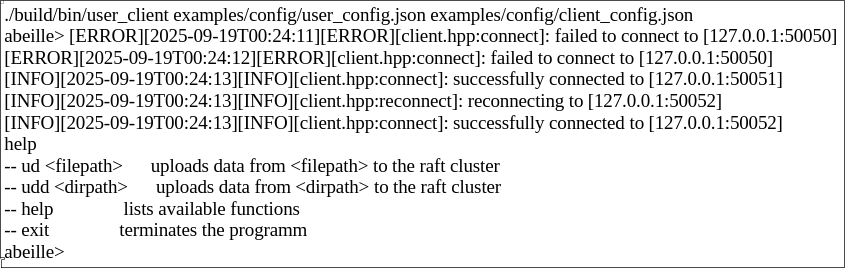
\includegraphics[width=0.8\linewidth]{inc/client-shell.png}
    \caption{Журнал запуска клиентского приложения: обработка недоступности узла и
    успешное подключение к кластеру.}
    \label{fig:client_start}
\end{figure}

После установления соединения клиент переходит в интерактивный режим, предлагая
пользователю список доступных команд. В частности, доступны функции загрузки
данных из файла или директории (\texttt{ud}, \texttt{udd}), вывод справочной
информации и завершение работы программы. На этом этапе система готова к
приёму задания и дальнейшему тестированию логики репликации и обработки задач.

\subsubsection{Запуск вычислительных узлов и их подключение к кластеру}

После инициализации клиентской части производится запуск вычислительных узлов,
которые будут непосредственно выполнять задачи.Логи на
рис.~\ref{fig:worker_start} демонстрируют, что, как и в случае с клиентом,
рабочий узел поочерёдно пытается подключиться к указанным в
\texttt{client\_config.json} узлам. Первая пара попыток к
\texttt{127.0.0.1:50050} завершилась ошибкой соединения, после чего рабочий
переключился на следующий адрес и успешно установил потоковое RPC-соединение с
\texttt{127.0.0.1:50051}, а затем и с лидером \texttt{127.0.0.1:50052}.

\begin{figure}[h!]
    \centering
    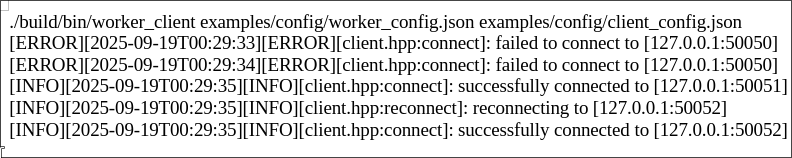
\includegraphics[width=0.8\linewidth]{inc/worker-log.png}
    \caption{Логи запуска вычислительного узла: автоматический обход узлов и успешное подключение.}
    \label{fig:worker_start}
\end{figure}

После установления соединения рабочий переходит в состояние \texttt{IDLE},
публикуя свой статус в поток \texttt{WorkerService.Connect}, что позволяет
кластеру учитывать его при назначении новых задач. Таким образом, уже на этом
этапе проверяется важная функциональность системы — автоматический выбор
доступного узла и готовность рабочего принимать задания от лидера кластера.

\subsubsection{Тестирование выполнения задания}

Для проверки корректности работы системы был проведён end-to-end тест с
использованием простого вычислительного задания. В качестве тестовой функции
был выбран алгоритм факторизации числа на простые множители, реализованный на
C++. Такая задача является хорошим примером для функционального тестирования:
она не требует сложной подготовки данных, но даёт детерминированный и легко
проверяемый результат. Код задания представлен в приложении В. В качестве
входных данных подавались 10000 чисел.

Постановка задачи выполнялась из интерактивной консоли клиентского приложения с
помощью команды \texttt{ud}, передающей содержимое \texttt{data.json} в
кластер. Это представлено на рис.~\ref{fig:client-send}. Клиент подтвердил
успешную загрузку данных, а после обработки задачи вывел сообщение о получении
результата.

\begin{figure}[h!]
    \centering
    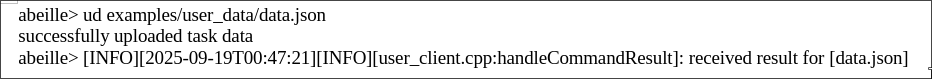
\includegraphics[width=0.8\linewidth]{inc/client-send.png}
    \caption{Процесс пересылки данных на клиенте}
    \label{fig:client-send}
\end{figure}

На стороне лидера Raft логи показан полный путь задачи: назначение её
конкретному рабочему узлу, репликацию соответствующей команды в Raft-лог, достижение
кворума и коммит, а также последующую фиксацию результата (см.
рис.~\ref{fig:master-log-task}). При этом реплика синхронизировалась с лидером,
что видно по сообщениям \texttt{HandleAppendEntry} и обновлению индексов
коммита (см. рис.~\ref{fig:replica-log-task}).

\begin{figure}[h!]
    \centering
    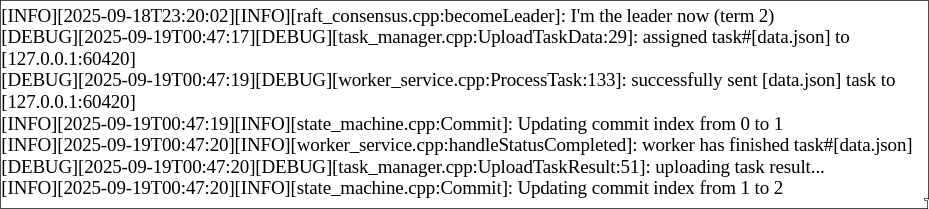
\includegraphics[width=0.8\linewidth]{inc/master-log-task.png}
    \caption{Лог мастера при назначении задания}
    \label{fig:master-log-task}
\end{figure}

\begin{figure}[h!]
    \centering
    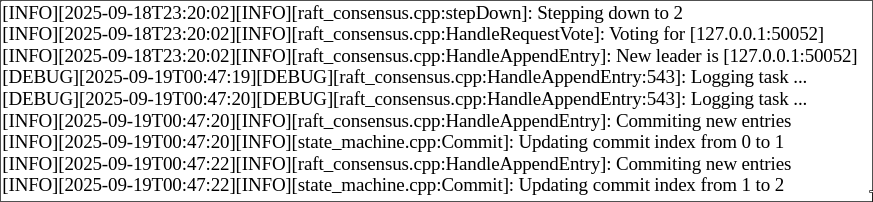
\includegraphics[width=0.8\linewidth]{inc/replica-log-task.png}
    \caption{Лог реплики при назначении задания}
    \label{fig:replica-log-task}
\end{figure}

Логи вычислительного узла подтвердили успешное получение задания: рабочий узел перешёл
в состояние \texttt{BUSY}, инициировал локальный процесс обработки данных
через IPC, корректно завершил вычисление и вернул результат обратно в кластер
(см. рис.~\ref{fig:worker-log-task}).

\begin{figure}[h!]
    \centering
    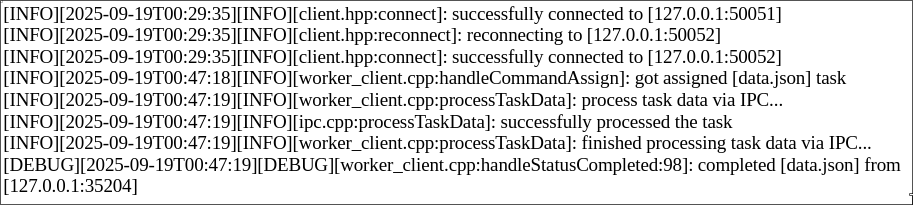
\includegraphics[width=0.8\linewidth]{inc/worker-log-task.png}
    \caption{Лог вычислительного узла при выполнении работы}
    \label{fig:worker-log-task}
\end{figure}

На стороне мастера была зафиксирована команда \texttt{RAFT\_COMMAND\_MOVE},
переведшая задачу в статус завершённой, после чего результат был передан
пользовательскому клиенту. Таким образом, в рамках теста была проверена вся
цепочка обработки: от приёма входных данных до финализации состояния в машине
состояний и возврата результата.

Проведённый эксперимент подтверждает корректность реализации основных
механизмов системы: клиентские запросы реплицируются и коммитятся только при
достижении кворума, рабочие получают задачи и публикуют статус их выполнения,
а пользователь всегда наблюдает согласованное состояние кластера, даже при
ранее проведённых сменах лидера или мертвых узлах.

\subsubsection{Нагрузочный тест с 50 параллельными клиентами}

Для проверки поведения системы при высокой конкурентной нагрузке был
организован сценарий с одновременной работой пятидесяти клиентских процессов.
Каждый клиент открывал двунаправленное gRPC-соединение с кластером, отправлял
одну команду \texttt{ud} для постановки задачи в очередь и завершал работу,
освобождая слот для следующих запусков. Параллельный запуск был реализован
средствами утилиты \texttt{GNU parallel} (см. рис.~\ref{fig:leader-multi-conn}),
обеспечивающей одновременный запуск 50 процессов с минимальной задержкой между
стартами.

\begin{figure}[h!]
    \centering
    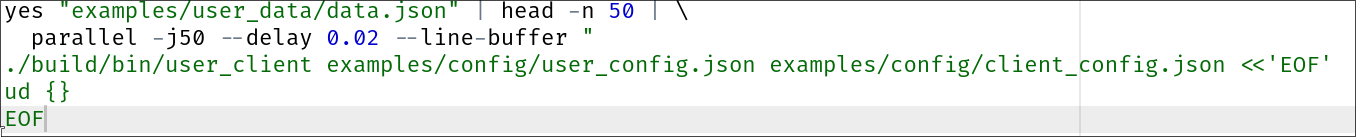
\includegraphics[width=0.95\linewidth]{inc/load-multi.png}
    \caption{Нагрузочный тест}
    \label{fig:leader-multi-conn}
\end{figure}

В данном тесте использовались два рабочих узла. Кластер Raft выбрал
лидера в начале прогона, после чего последовательно обрабатывал поступающие
задания. В журнале лидера наблюдается монотонное увеличение индекса коммита
каждой новой записи лога (рис.~\ref{fig:leader_log_50}), что подтверждает
корректную репликацию команд и достижение кворума. Каждое успешно завершённое
задание сопровождается сообщением
\texttt{worker\_service.cpp:handleStatusCompleted}, после чего в машине
состояний фиксируется переход задачи из состояния \texttt{assigned} в
\texttt{completed}.

\begin{figure}[h!]
    \centering
    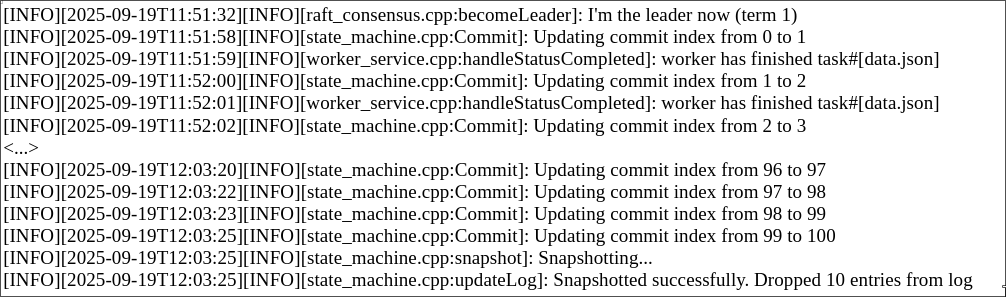
\includegraphics[width=0.95\linewidth]{inc/leader-multi-conn.png}
    \caption{Фрагмент лога лидера во время нагрузочного теста с 50 клиентами}
    \label{fig:leader_log_50}
\end{figure}

При достижении сотого коммита сработал механизм создания снимка данных, что
подтверждается сообщением \texttt{Snapshotting...} в логах. После успешного
сохранения состояния машины состояний на диск (\texttt{Snapshotted
successfully}) из лога были удалены 10 записей, как и предусмотрено параметром
\texttt{snapshot\_after} в конфигурации. Продолжение работы кластера после
создания снимка данных не вызвало увеличения задержек или ошибок репликации, что
свидетельствует о корректности реализации механизма архивации и его
прозрачности для клиентских приложений.

Таким образом, тест показал, что система способна обрабатывать десятки
одновременных подключений, сохраняя линейризуемость состояния и выполняя
своевременное архивирование лога без нарушения доступности сервиса.

\subsubsection{Тестирование на задаче с большим объёмом данных}

Для проверки корректности работы системы при выполнении ресурсоёмких задач был
проведён эксперимент с входными данными увеличенного размера (около двух
миллионов элементов). Задача была отправлена в кластер с использованием
стандартного клиента и поступила на один из доступных рабочих узлов. Фрагмент
лога рабочего узла приведён на рис.~\ref{fig:worker_bigdata}.

\begin{figure}[h!]
    \centering
    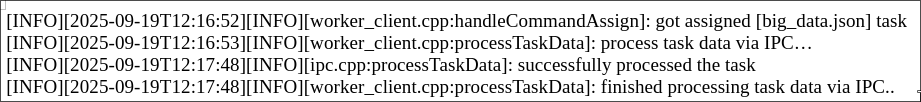
\includegraphics[width=0.95\linewidth]{inc/worker-big-data.png}
    \caption{Лог вычислительного узла при обработке задачи с 2 млн элементов}
    \label{fig:worker_bigdata}
\end{figure}

Как видно из лога, узел получил команду назначения задачи
(\texttt{handleCommandAssign}), после чего перешёл к фазе обработки данных через
IPC-механизм (\texttt{processTaskData}). Общая длительность обработки составила
около 56 секунд, что соответствует ожидаемому времени выполнения для задачи
данного объёма. По завершении вычислений задача была успешно отмечена как
выполненная (\texttt{finished processing task data via IPC}), а результат был
передан обратно в кластер и зафиксирован в машине состояний.

Данный эксперимент подтвердил, что система корректно обрабатывает задачи
увеличенной сложности и объёма, при этом не теряя связи с кластером и
сохраняя линейризуемость состояния. В течение всего времени выполнения других
ошибок или повторных назначений задачи не наблюдалось, что демонстрирует
устойчивость и надёжность реализации даже при продолжительных вычислениях.
